\documentclass{beamer}
\usetheme{Montpellier}
\usefonttheme[onlylarge]{structurebold}
\setbeamerfont*{frametitle}{size=\normalsize,series=\bfseries}
\setbeamertemplate{navigation symbols}{}

\useoutertheme{infolines}

\usepackage{mathtools}
\DeclarePairedDelimiter{\ceil}{\lceil}{\rceil}

\usepackage[english]{babel}
\usepackage[latin1]{inputenc}
\usepackage[T1]{fontenc}

\long\def\/*#1*/{}

\title[COOJA-UDGO]
{
  Simulando redes sem-fio com obst�culos usando o COOJA extendido
}
\author[Manass�s]
{
  Manass�s~Ferreira\inst{1} \\
  {\scriptsize
  mfer@dcc.ufmg.br
  }
}
\institute[UFMG]
{
  \inst{1}
Departamento de Ci�ncia da Computa��o\\
Universidade Federal de Minas Gerais (UFMG)\\
Belo Horizonte, Brazil
}
\date[\today]
{ 
  Projeto Orientado em Computa��o - 2014/2\\
  {\scriptsize
  {\bf Professor}: Clodoveu Davis {\it e} Marcos Andr� Gon�alves \\
  {\bf Orientador}: Olga Goussevskaia \\
  \{clodoveu, mgoncalv, olga\}@dcc.ufmg.br  
  }
}

\begin{document}

  \begin{frame}
    \titlepage
  \end{frame}

  \begin{frame}{Agenda}
    \tableofcontents
  \end{frame}

  \section{Trabalho Relacionado}
    \subsection{COOJA - Contiki}  
      \begin{frame}{Simulador e SO}
        \begin{columns}
          \begin{column}{.5\linewidth}
            \begin{figure}[h!]
              \centering
                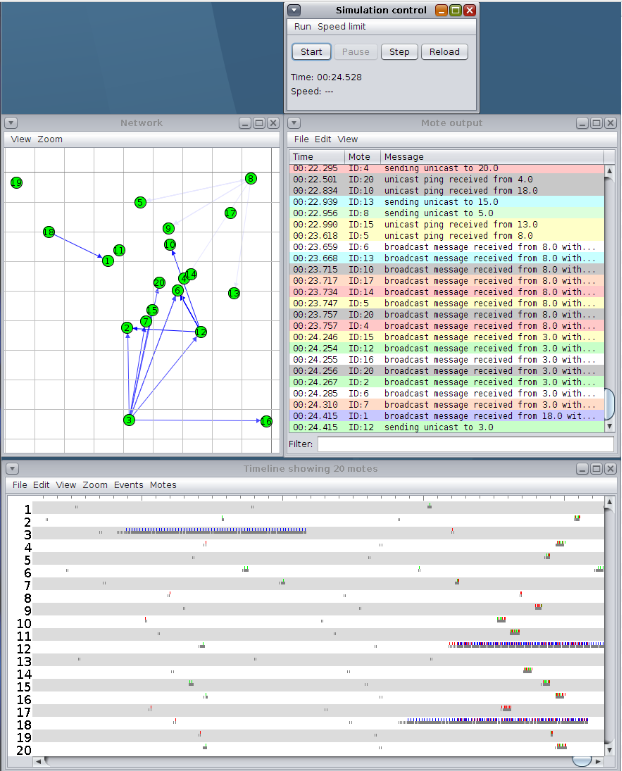
\includegraphics[width=1\textwidth]{img/cooja.png}
            \end{figure}   
          \end{column}
          \begin{column}{.5\linewidth}
            \begin{figure}[h!]
              \centering
                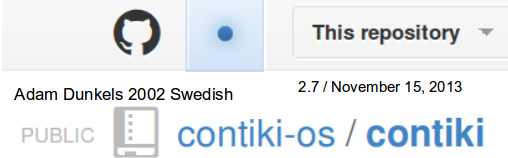
\includegraphics[width=1\textwidth]{img/contiki.png}
            \end{figure}   
          \end{column}
        \end{columns}
      \end{frame}
      
    \subsection{Redes sem-fio com obst�culos}  
      \begin{frame}{Modelo}
        \begin{figure}[h!]
          \centering
            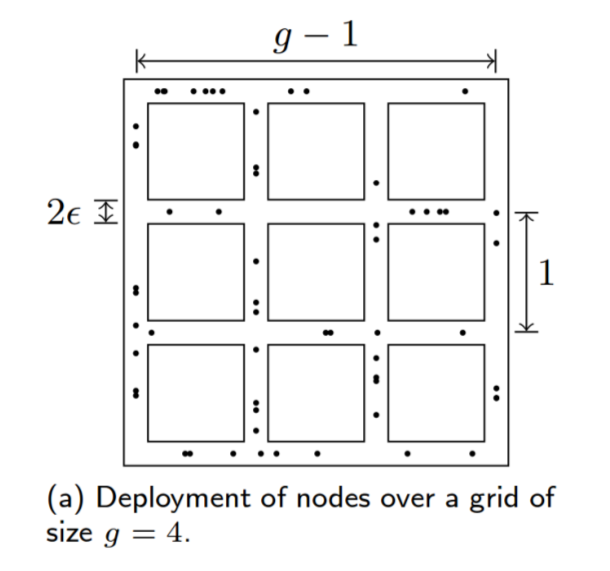
\includegraphics[width=0.6\textwidth]{img/model.png}
        \end{figure}   
      \end{frame}
      \begin{frame}{Raio Cr�tico de Transmiss�o}
        \begin{figure}[h!]
          \centering
            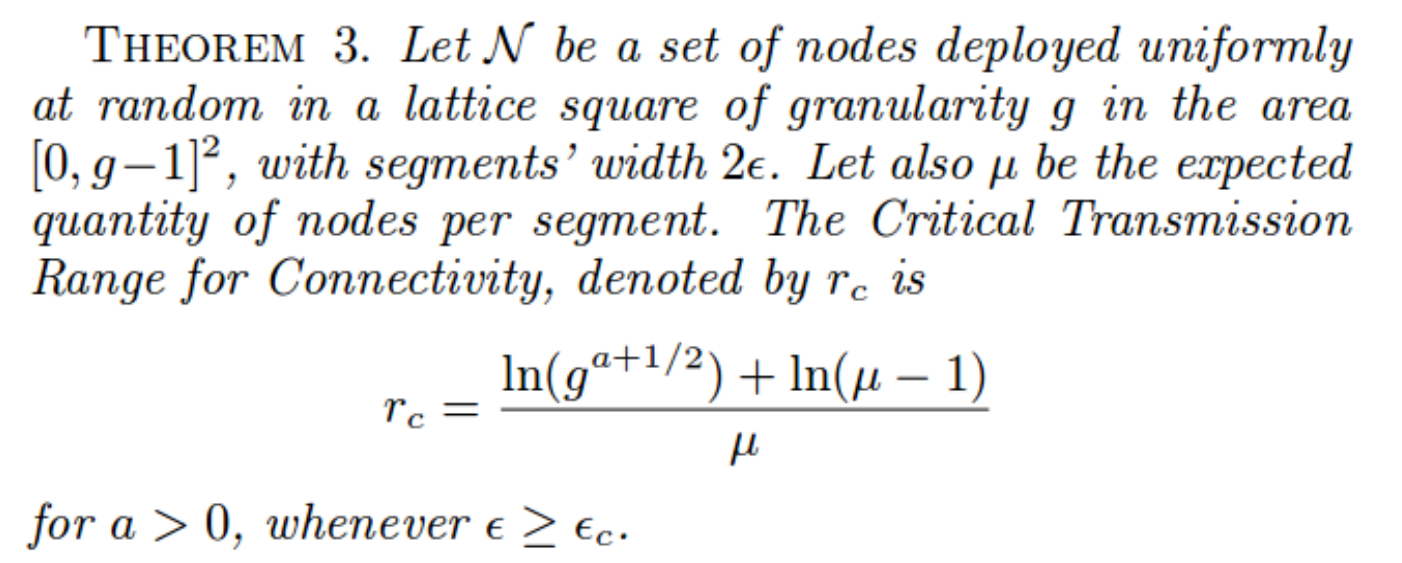
\includegraphics[width=1\textwidth]{img/ctr-analytical.png}\\
            {a=1}
        \end{figure}   
      \end{frame}

  \section{Trabalho Desenvolvido}
    \subsection{UDGO}  
      \begin{frame}{UDGM $\land$ MRM}
        \begin{figure}[h!]
          \centering
            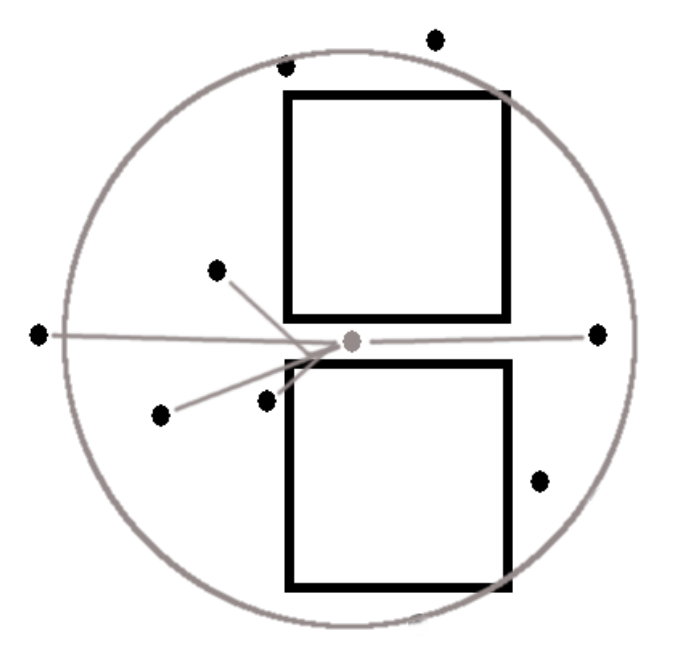
\includegraphics[width=0.6\textwidth]{img/udgo.png}
        \end{figure}   
      \end{frame}
    \subsection{Automa��o e An�lise}  
      \begin{frame}{Ciclo de Simula��o}
        \begin{figure}[h!]
          \centering
            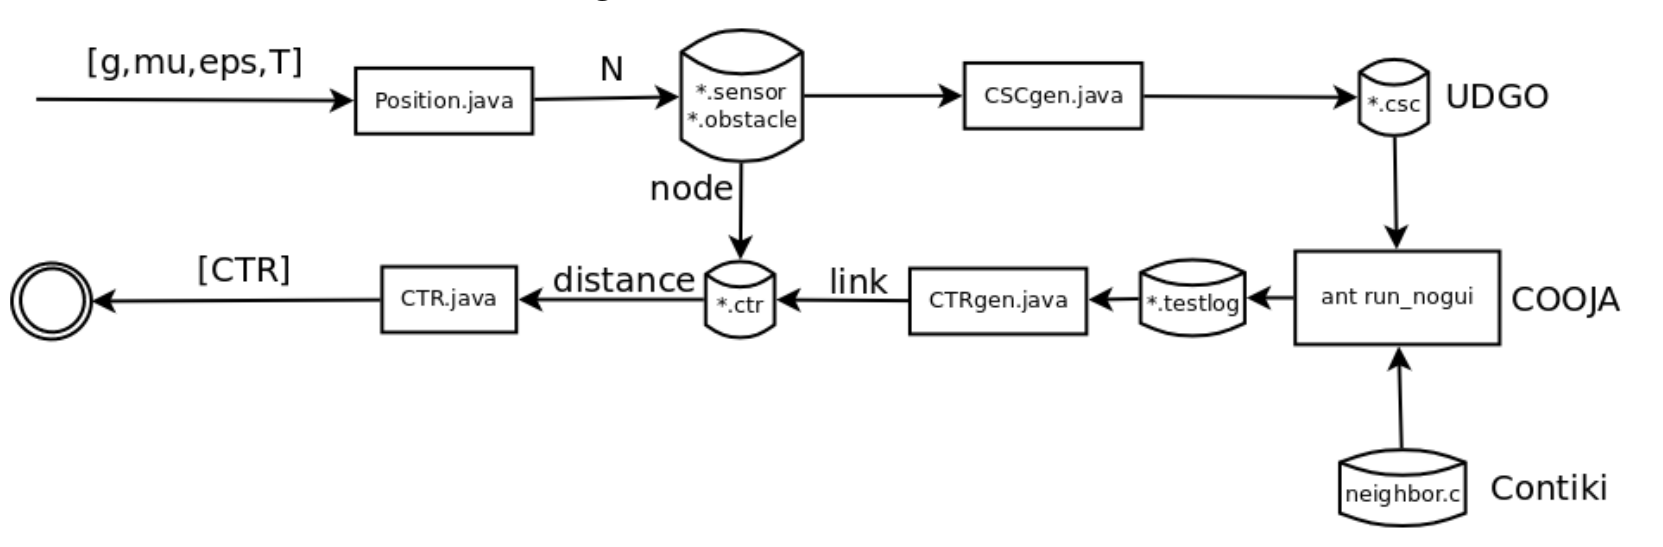
\includegraphics[width=1\textwidth]{img/simula-cycle.png}
        \end{figure}   
      \end{frame}
    \subsection{Computa��o distribu�da}  
      \begin{frame}{Protocolo Cliente-Servidor}
        \begin{figure}[h!]
          \centering
            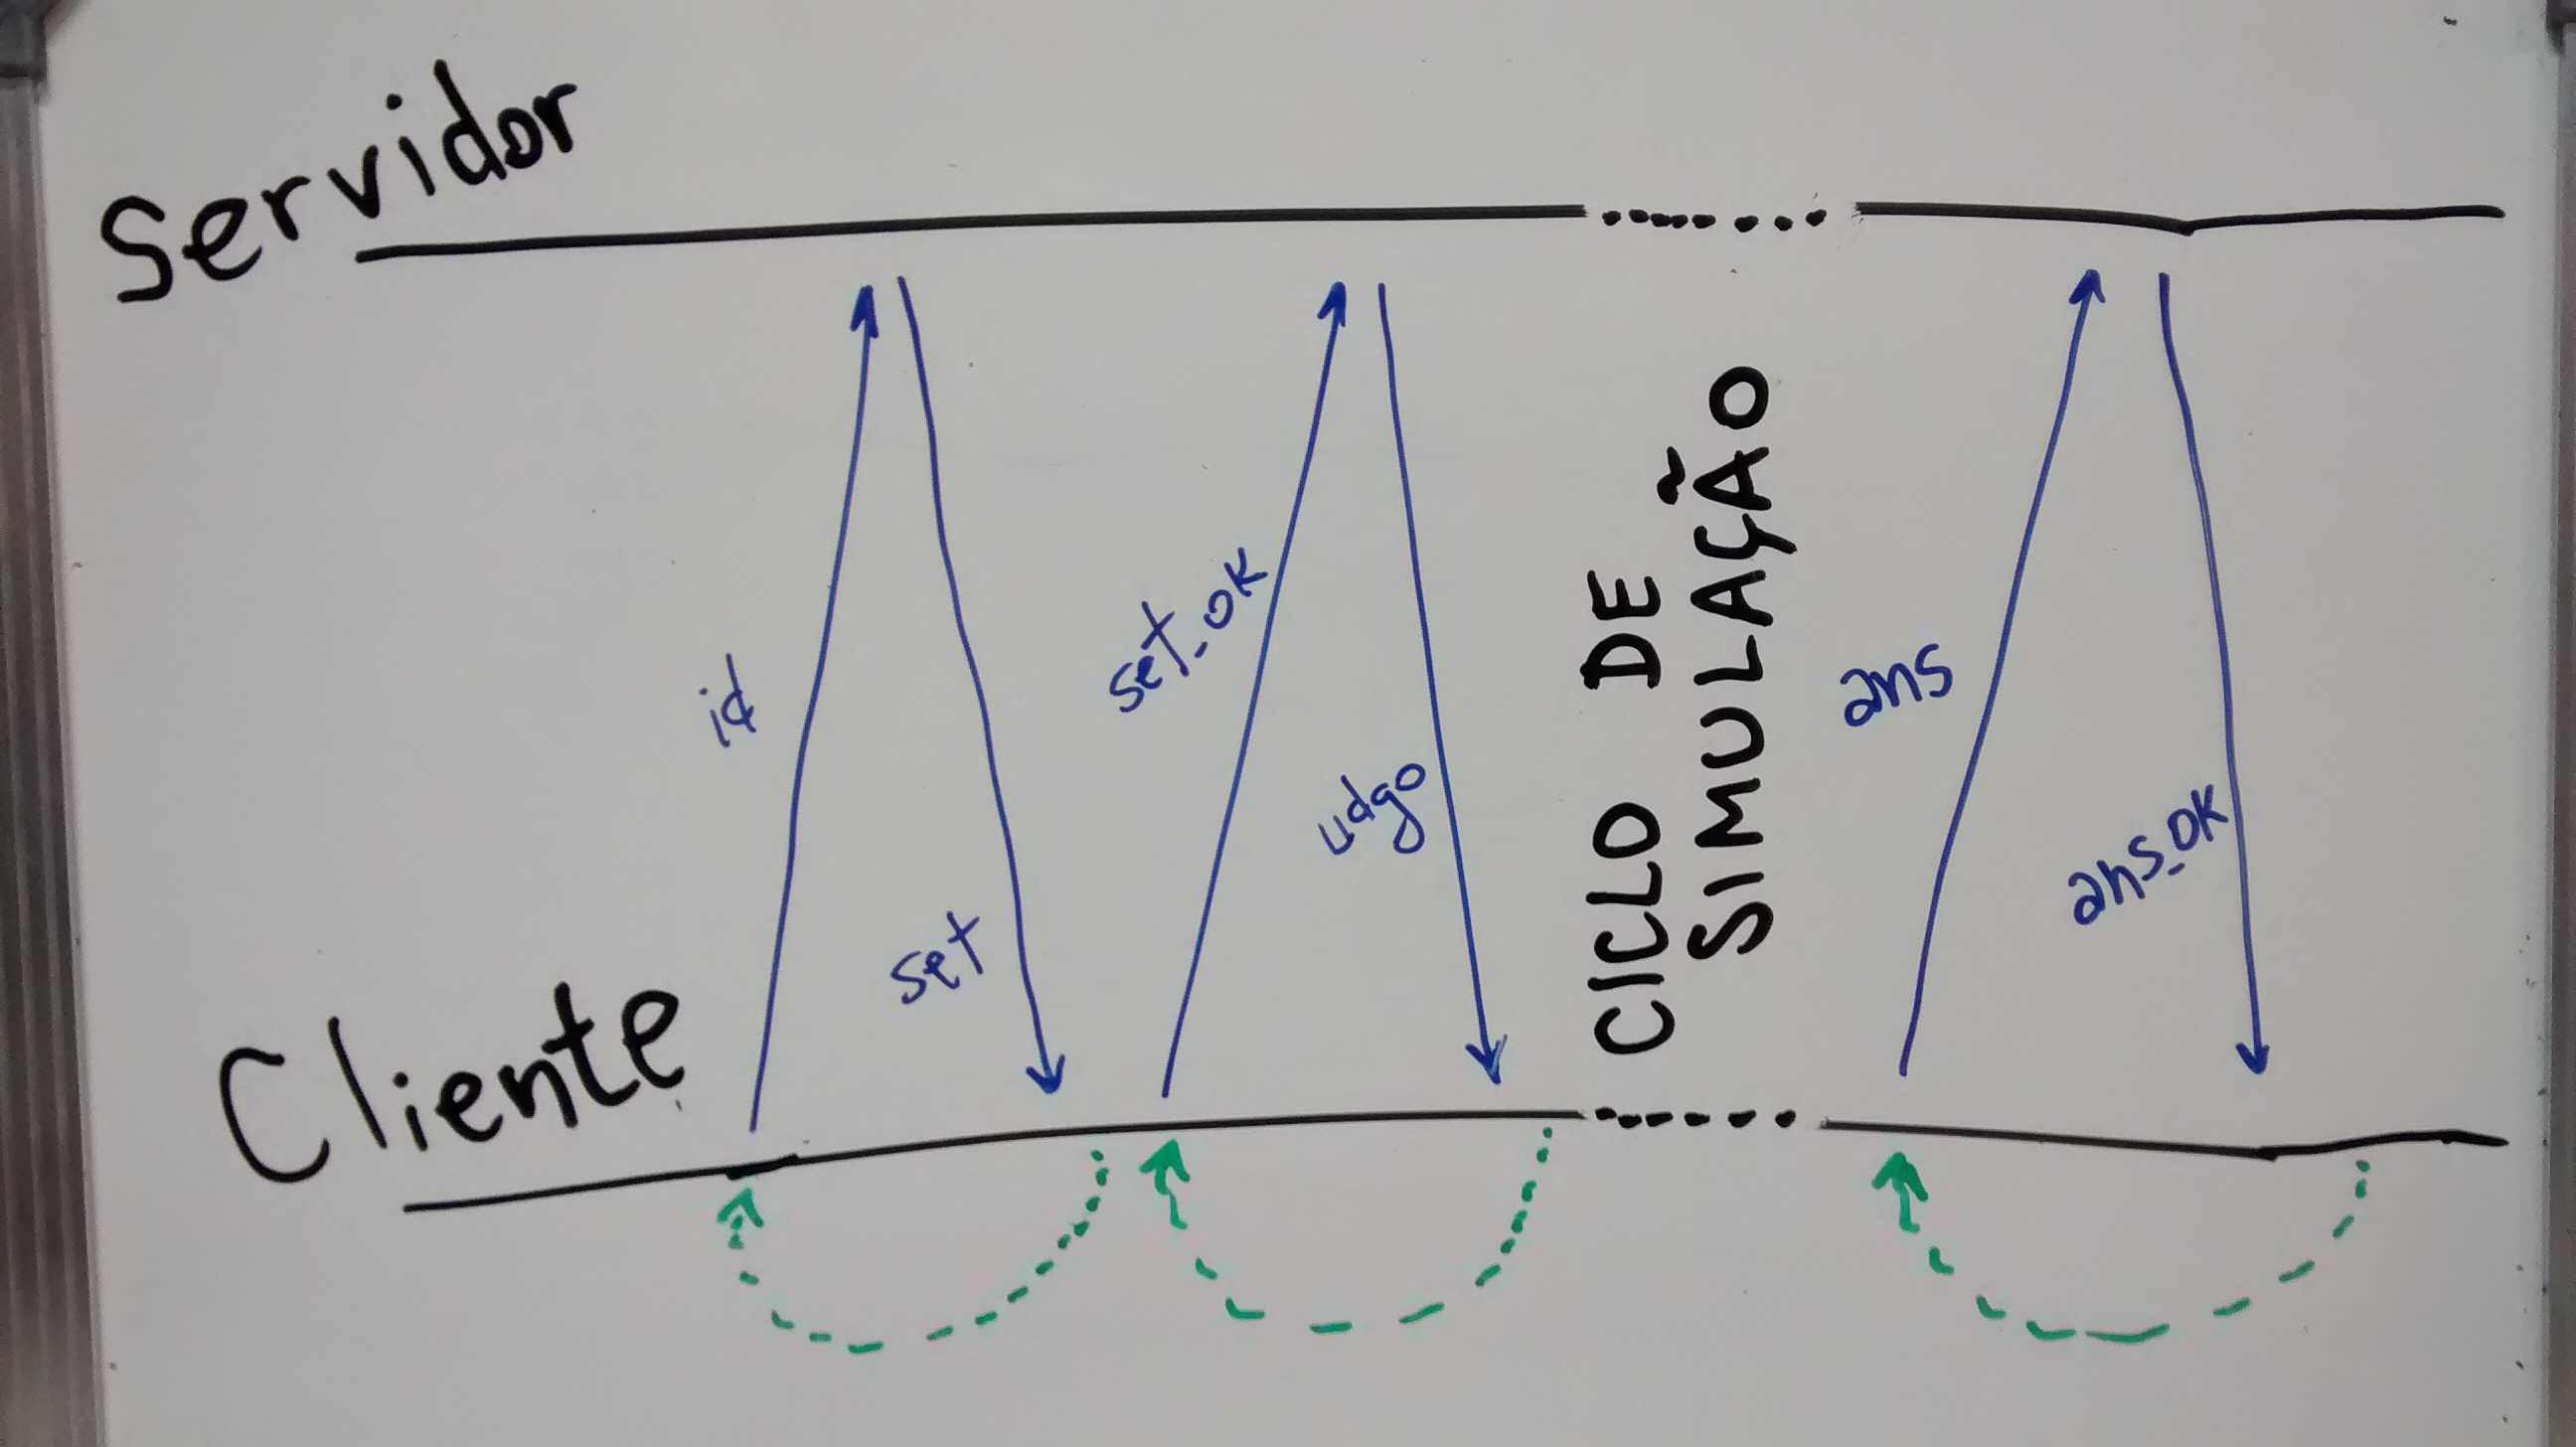
\includegraphics[width=1\textwidth]{img/client-server.jpg}
        \end{figure}   
      \end{frame}

  \section{Resultado}
    \subsection{Esperado}  
      \begin{frame}{Insights}
        \begin{enumerate}
          \item Como o modelo poderia ser 'alimentado' pelo meio f�sico UDGO?\\
          \item CTR experimental ser� menor que o anal�tico?\\
          \item Propriedades f�sicas do MRM podem aumentar visibilidade? E a interfer�ncia?
        \end{enumerate}
      \end{frame}    
    \subsection{Pr�via}  
      \begin{frame}{Inst�ncia Pequena}
        \begin{figure}[h!]
          \centering
            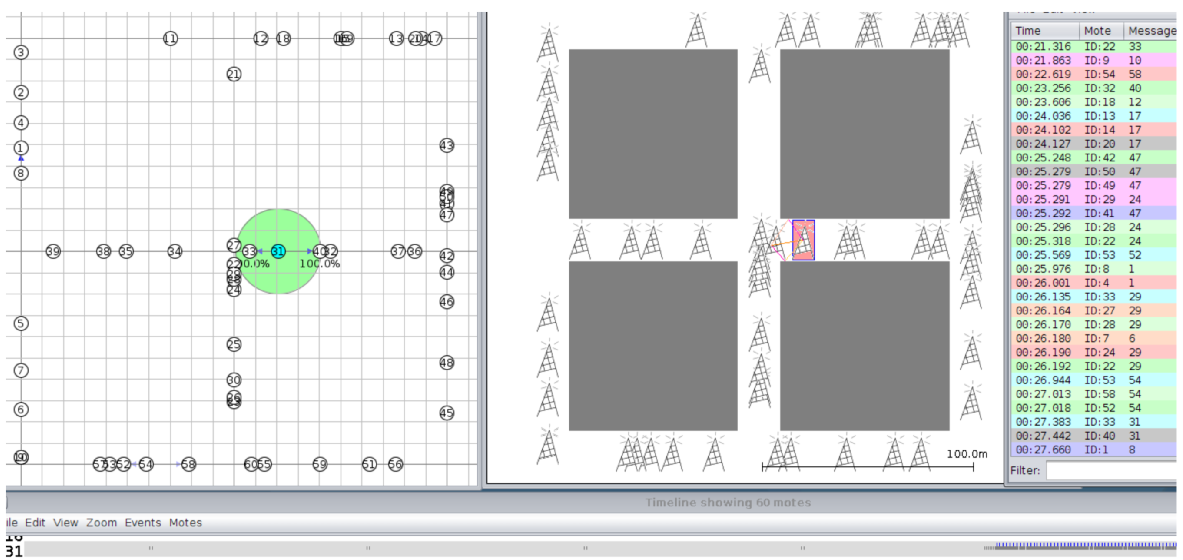
\includegraphics[width=1.0\textwidth]{img/one-example.png}\\
            {$T=20$, $g=3$, $\mu=5$, $\epsilon=10$}\\
            {$CTR_{experimental}=19.96$}\\
            {$r_{c}=46.82$}
        \end{figure}   
      \end{frame}    

  \section{Trabalho por Desenvolver}
    \subsection{Gerar Resultados}  
      \begin{frame}{Inst�ncias Maiores}
        \centering

\begin{tabular}{l*{7}{c}r}
\hline
T            & 20 & 30 & 35 & 28 & 70 \\
\hline
g            & 2 & 6 & 8 & 12 \\
\hline
$\mu$        & 6 & 8 & 10 & 12 &  14 & 16 &  18  \\
\hline
$\epsilon$   & 10  \\
\hline
\end{tabular}

      \end{frame}    
    \subsection{Diminuir tempo de simula��o otimizando COOJA}  
      \begin{frame}{Um modo mais eficiente de computar visibilidade}
        \begin{figure}[h!]
          \centering
            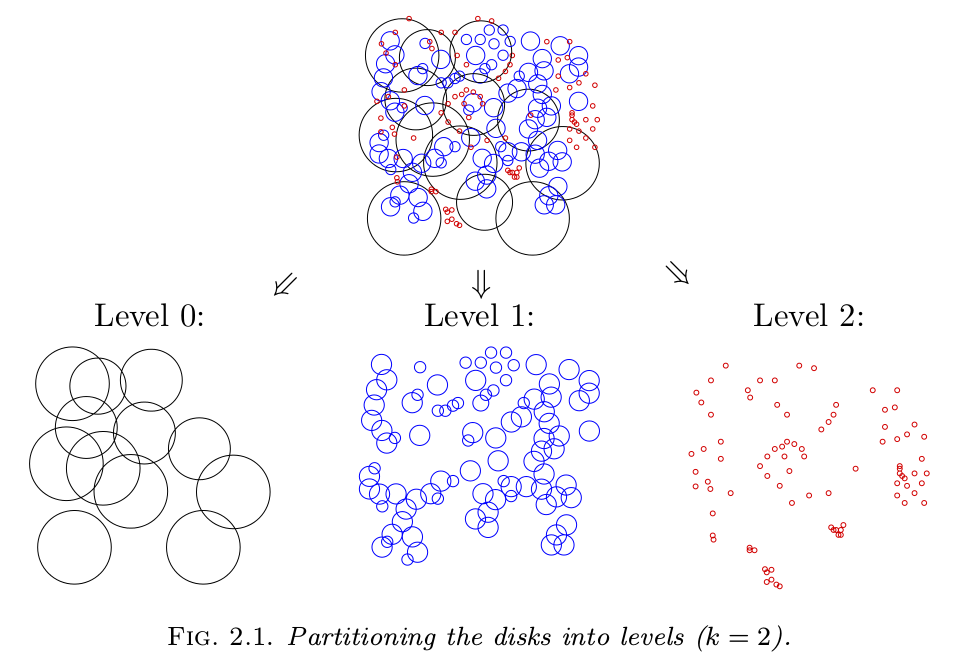
\includegraphics[width=0.5\textwidth]{img/2-1-fig.png}\\
            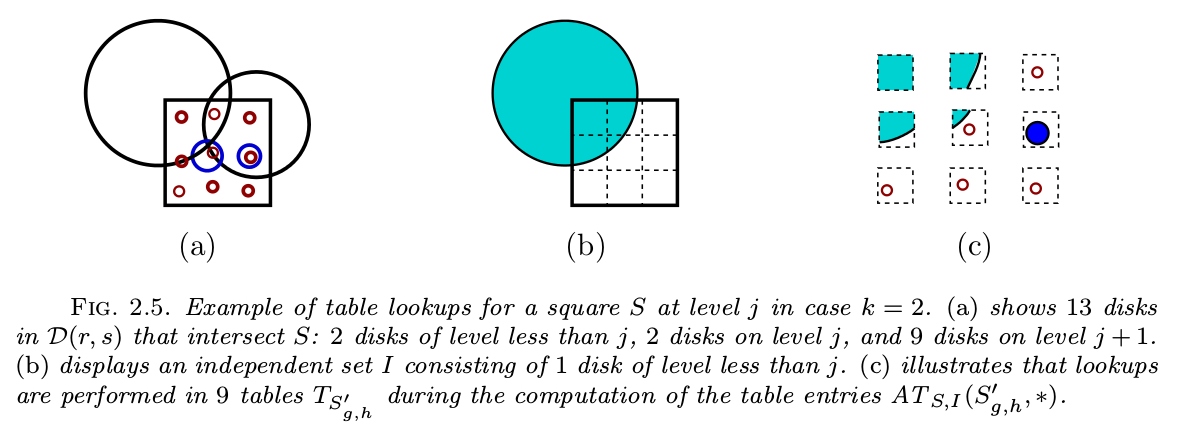
\includegraphics[width=0.6\textwidth]{img/2-5-fig.png}\\
            Ideia: 'Estrat�gia Deslocadora'
        \end{figure}
        
      \end{frame}    


  \section{}
    \subsection{}  
      \begin{frame}{Perguntas}
        \begin{figure}[h!]
          \centering
            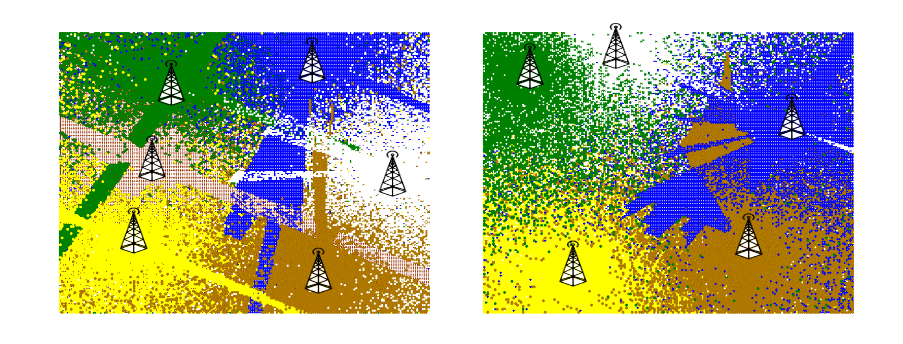
\includegraphics[width=1.0\textwidth]{img/callControl.png}
        \end{figure}   
      \end{frame}    

\end{document}
